\subsection{Methods and Analysis}

\subsubsection{Formalizing the FAM}
\label{section:transition_models}

Let $\mathcal{M}$ denote a set of possible health states, some of which can be absorbing. Transition times are ages of measurement. Let $\mathcal{A}:= [ 0, \ldots, \bar{A}]$ index ages, where $\bar{A}$ is the last age that we forecast. We define $h_{a,m,m'}$ as the probability of transitioning from state $m$ to state $m'$ at age $a \in \mathcal{A}$, where $m, m' \in \mathcal{M}$. We drop individual subscripts to avoid notational clutter.

We denote a state transition from $m$ to $m'$ at age $a$ by $D_{a,m,m'} = 1$. If this transition does not happen,  $D_{a,m,m'} = 0$. We let $\tilde{D}_{a,m}$ be the indicator of occupancy of state $m$ at age $a$. $\tilde{D}_{a,m} = 0$ otherwise. $\tilde{D}_{a,m}$ is a generic entry in the the vector of age-$a$ state occupancy indicators denoted by $\tilde{\bm{D}}_a$. $\tilde{\bm{D}}_0$ denotes the vector of initial state-occupancy conditions.

The general framework in \citet{Heckman_1981_heterogeneity,Heckman_1981_IncidentalParametersProblem} models the transition probability from state $m$ to state $m'$ at age $a$, $h_{a,m,m'}$, as being generated by the following index threshold-crossing model:
\begin{eqnarray}
I_{a,m,m'} &=& \bm{Z_a} \bm{\beta}_{a,m,m'} + \tau \left( a \right)_{m,m'} + \varepsilon_{a,m,m'}, \label{eq:trans0}
\end{eqnarray}
where $D_{a,m,m'} = \bm{\mathit{1}}  \left( I_{a,m,m'} \geq 0 \right)$, $\bm{Z_a}$ is a vector of covariates with associated coefficient vector $ \bm{\beta}_{a,m,m'}$, $\tau \left( a \right)_{m,m'}$ is a function of age, and $\varepsilon_{a,m,m'}$ is a general time-varying age-$a$ shock. This is a model of state transitions. In the framework of  \citet{Heckman_1981_heterogeneity,Heckman_1981_IncidentalParametersProblem}, this model is supplemented with initial conditions and survival models.

We simplify the complex reality of having to precisely describe each of the health states and how different competing risks generate them by modeling state occupancies and simplifying states to be, as a starting point, diseases that we separately model and then simulate. We then clarify how this model is adapted to other health and economic outcomes. Examples of these other outcomes include smoking, body-mass index, and binge drinking.

The probability of occupying a state $m \in \mathcal{M}$ at age $a \in{A}$ is generated by an index threshold-crossing model:
\begin{eqnarray}
I_{a,m} &=&  \bm{\mathit{1}} \left( \tilde{\bm{D}}_{0} \geq 0 \right) \bm{\Omega}_{m} + \bm{\mathit{1}} \left( \tilde{\bm{D}}_{a-1} \geq 0\right) \bm{\Lambda}_{m} + \bm{W_a} \bm{\beta}_{m} + \bm{B} \bm{\alpha}_m + \tau(a)_m + \varepsilon_{a,m}, \label{eq:trans}
\end{eqnarray}
where $\tilde{D}_{a,m} = \bm{\mathit{1}}  \left( I_{a,m} \geq 0 \right)$, $\tau \left( a \right)_{m}$ is a function of age,\footnote{In our empirical analysis, we approximate the coefficients on $\tau \left( a \right)_{m}$ using splines with knots at ages 35, 45, 55, 65, and 75.} and $\varepsilon_{a,m}$ is a time-varying age-$a$ shock, uncorrelated across ages, subjects, and health states. As in the forecasts of Section~\ref{section:cbamethodology}, we allow the model to depend on baseline variables, denoted by $\bm{B}$, and on variables that can be affected by treatment, which in this case we denote by $\bm{W}_a$ to reinforce that they are not the same variables that we use in Section~\ref{section:cbamethodology}. The variables in $\bm{W}_a$ contain health outcomes and other economic outcomes (e.g.,\ smoking, labor force participation, childrearing). $ \bm{\Omega}_{m},  \bm{\Lambda}_{m}, \bm{\beta}_{m},  \bm{\alpha}_{m}$ are the coefficient vectors associated with the initial state-occupancy indicators, first-order lagged state-occupancy indicators, current health and other economic outcomes, and baseline variables. In our empirical analysis, we estimate these vectors for each state occupancy $m \in \mathcal{M}$.

Instead of supplementing the model in Equation~\eqref{eq:trans} with a model for initial conditions, we directly condition on them in Equation~\eqref{eq:trans}. Uncorrelatedess of $\varepsilon_{a,m}$ across ages, health states, and subjects together with normality allows us to perform separate estimation of the coefficients characterizing Equation~\eqref{eq:trans} for each $m \in \mathcal{M}$ using maximum likelihood. We estimate $\bm{\theta}_m := \left[   \bm{\Omega}_{m}, \bm{\Lambda}_{m}, \bm{\beta}_{m}, \alpha_{m}, \tau \left( a \right) _{m}  \right]$ for each $m \in \mathcal{M}$.

Despite the many simplifications on the definition of health states and on modeling state occupancies instead of state transitions, Appendix~\ref{appendix:health-validation} documents that our procedure performs well at fitting populations means of the outcomes that we consider.

The probability of occupying states is estimated in FAM from Equation~\eqref{eq:trans}. When simulating the model to forecast the health outcomes for the ABC/CARE subjects, we use their observed age-30 conditions as initial conditions  $\tilde{\bm{D}}_0$. The majority of these initial conditions relate to health, but we also include economic initial conditions. The simulation proceeds in an analogous fashion to the simulation in Section~\ref{section:cbamethodology}---in which case we initialize the forecast with age-21 labor income. The vector $\tilde{\bm{D}}_0$ could have been affected by treatment. \citet{Campbell_Conti_etal_2014_EarlyChildhoodInvestments} estimate the wide variety of effects on health outcomes that ABC/CARE had. This motivates the inclusion of health outcomes into our analysis.

We use modified versions of Equation~\eqref{eq:trans} to model the following additional health states and outcomes.

\begin{enumerate}
\item \textbf{Absorbing states.} An absorbing state is a state $m \in \mathcal{M}$ such that once a subject occupies that state he/she never abandons it. That is, $m \in \mathcal{M}$ is an absorbing state if $\tilde{D}_{a,m} = 1$ implies that $\tilde{D}_{a',m} = 1 \ \forall a' \in \mathcal{A}$ with $a' \geq a.$ Once an individual reaches an absorbing stage his/her posterior observations are dropped from the estimation of Equation~\eqref{eq:trans}. An obvious example of an absorbing state is death.
\item \textbf{Ordered and unordered threshold models.} Ordered and unordered outcomes are outcomes for which a multiple-threshold model is employed as a straightforward modification to Equation~\eqref{eq:trans}. An example of the former is the level of psychological distress (e.g.,\ low, medium, high). An example of the latter is labor force status (e.g., labor force status is categorized as out of labor force, unemployed, working part time, or working full time).
\item \textbf{Continuous outcomes modeled as linear models.} An example of a continuous outcome is body-mass index (BMI).
\end{enumerate}

Estimation of the parameters characterizing these outcomes is also performed separately. The economic outcomes that we include are labor income, for which we use the forecast detailed in Section~\ref{section:cbamethodology}, as well as labor force participation, relationship status, and childbearing. 

Tables~\ref{table:supertab1} to~\ref{table:supertab3} list the variables determining each of the states and health and economic outcomes that we consider. For each of these we list: (1) the outcome; (2) the variable type---e.g., absorbing state, binary outcome, continuous outcome; (3) initial health state occupancies and other other outcomes---$\tilde{\bm{D}}_0$ in Equation~\eqref{eq:trans}; (4) lagged health-state occupancies---$\tilde{\bm{D}}_{a-1}$ in Equation~\eqref{eq:trans}; (5) and (6) other health and economic outcomes used to determine the outcome of interest---$\bm{W}_a$ in Equation~\eqref{eq:trans}; and (7) background variables---$\bm{B}$ in Equation~\eqref{eq:trans}. From this information, the reader can understand the type of outcome being model, its classification, as well as determinants and their categorization according to Equation~\eqref{eq:trans}. The outcomes that help predict each other are based on research and advice of clinicians and other medical professionals, as explained and justified in \citet{Goldman_etal_2015_Future-Elderly-Model-Report}.

% ABSORBING STATES
\begin{sidewaystable}[htbp!]
\caption{Determinants of Equation~\eqref{eq:trans}, 1/3} \label{table:supertab1}
\begin{scriptsize}
\begin{tabular}{lllllll}
\toprule 
\multicolumn{1}{c}{(1)} & \multicolumn{1}{c}{(2)} & \multicolumn{1}{c}{(3)} & \multicolumn{1}{c}{(4)} & \multicolumn{1}{c}{(5)} & \multicolumn{1}{c}{(6)} & \multicolumn{1}{c}{(7)} \\
 & &  \multicolumn{1}{c}{$\tilde{\bm{D}}_0$} &  \multicolumn{1}{c}{$\tilde{\bm{D}}_{a-1}$} & \multicolumn{1}{c}{ $\bm{W}_a$ } &  \multicolumn{1}{c}{ $\bm{W}_a$ } &  \multicolumn{1}{c}{$\bm{B}$} \\ 
\multicolumn{1}{c}{Outcome} & \multicolumn{1}{c}{Variable Type} & \multicolumn{1}{c}{Initial Conditions} & \multicolumn{1}{c}{Other States} & \multicolumn{1}{c}{Health Outcomes} & \multicolumn{1}{c}{Economic Outcomes} & \multicolumn{1}{c}{Demographics} \\
\midrule
Heart Disease   & Absorbing & Childhood Economic Environment & Hypertension    & Smoking   &                                & Race \\
			    &           & Education & Diabetes & BMI &  & Ethnicity \\
			    &           & Asthma & & Physical Activity &  & Age \\
			    &           &        &  &  &  & Gender \\
\midrule			
Hypertension & Absorbing & Childhood Economic Environment & Diabetes    & Smoking   &                                & Race \\
&           & Education &  & BMI &  & Ethnicity \\
&           &  & & Physical Activity &  & Age \\
&           &        &  &  &  & Gender \\
\midrule			
Stroke & Absorbing & Childhood Economic Environment & Heart Disease    & Smoking   &                                & Race \\
&           & Education & Hypertension & BMI &  & Ethnicity \\
&           &  & Diabetes & Physical Activity &  & Age \\
&           &        & Cancer &  &  & Gender \\
\midrule		
Lung Disease & Absorbing & Childhood Economic Environment &   & Smoking   &                                & Race \\
&           & Education & & BMI &  & Ethnicity \\
&           & Asthma &  & Physical Activity &  & Age \\
&           &        &  &  &  & Gender \\
\midrule		
Diabetes  & Absorbing & Childhood Economic Environment &   & Smoking   &                                & Race \\
&           & Education &  & BMI &  & Ethnicity \\
&           &  &  & Physical Activity &  & Age \\
&           &        &  &  &  & Gender \\
\midrule		
Cancer & Absorbing & Childhood Economic Environment &     & Smoking   &                                & Race \\
&           & Education & & BMI &  & Ethnicity \\
&           &  &  & Physical Activity &  & Age \\
&           &        & &  &  & Gender \\
\midrule
Mortality & Absorbing & Education & Heart Disease & Smoking &  & Race \\
&&  & Hypertension & Binge Drinking  & & Ethnicity \\
&& & Stroke & & & Age \\
&& & Lung Disease & & & Gender \\
&& & Diabetes & & & \\
&& & Cancer & & & \\
&& & Functional Status & & & \\
\midrule	
Functional Status & Ordered & Childhood Economic Environment & Heart Disease & Smoking & & Race \\
			&& Education & Hypertension & BMI &  & Ethnicity \\
			&&  & Stroke & Physical Activity & & Age \\
			&&  &  Lung Disease & Functional Status & & Gender \\
			&&  & Diabetes &  &  & \\
			&&  & Cancer & & & \\
			&&  &   &  &  & \\
\midrule
Smoking & Binary & Childhood Economic Environment & Heart Disease  & BMI & & Race \\
& & Education &  Lung Disease & Binge Drinking & & Ethnicity \\
&  &  & Diabetes & Physical Activity  & & Age \\
&  & &  & Psychological Distress & & Gender \\
\bottomrule
\end{tabular}
\end{scriptsize}
\end{sidewaystable}

\begin{sidewaystable}[htbp!]
\caption{Determinants of Equation~\eqref{eq:trans}, 2/3} \label{table:supertab2}
\begin{scriptsize}
\begin{tabular}{lllllll}
\toprule 
\multicolumn{1}{c}{(1)} & \multicolumn{1}{c}{(2)} & \multicolumn{1}{c}{(3)} & \multicolumn{1}{c}{(4)} & \multicolumn{1}{c}{(5)} & \multicolumn{1}{c}{(6)} & \multicolumn{1}{c}{(7)} \\
 & &  \multicolumn{1}{c}{$\tilde{\bm{D}}_0$} &  \multicolumn{1}{c}{$\tilde{\bm{D}}_{a-1}$} & \multicolumn{1}{c}{ $\bm{W}_a$ } &  \multicolumn{1}{c}{ $\bm{W}_a$ } &  \multicolumn{1}{c}{$\bm{B}$} \\ 
\multicolumn{1}{c}{Outcome} & \multicolumn{1}{c}{Variable Type} & \multicolumn{1}{c}{Initial Conditions} & \multicolumn{1}{c}{Other States} & \multicolumn{1}{c}{Health Outcomes} & \multicolumn{1}{c}{Economic Outcomes} & \multicolumn{1}{c}{Demographics} \\
\midrule
BMI & Continuous & Childhood Economic Environment & & BMI & Marital Status & Race \\
& & Education & & & & Ethnicity \\
 & &  & & & & Age \\
 &  & & & & & Gender \\
\midrule
Binge Drinking & Binary & Childhood Economic Environment &  Marital Status & Binge Drinking & & Race \\
 & & Education &  &  & & Ethnicity \\
  & &  &  &  & & Age \\
  &  & &  &  & & Gender \\
\midrule
Physical Activity & Binary & Childhood Economic Environment & Marital Status & Physical Activity & & Race \\
 & & Education &  & & & Ethnicity \\
  & &  &  &  & & Age \\
  &  & &  &  & & Gender \\
\midrule
Psychological Distress & Ordered & Childhood Economic Environment & Heart Disease & Smoking & & Race \\
 & & Education & Hypertension & BMI & & Ethnicity \\
 &  &  & Stroke & Physical Activity & & Age \\
   & & & Lung Disease & Psychological Distress & & Gender \\
    & & & Diabetes & Functional Status & & \\
     & & & Cancer & & & \\
\midrule		
Childbearing & Ordered & Mother's Education  & Cancer & Marital Status & Labor Force Participation & Race \\
&  & Education  & & & Number of Children & Ethnicity \\
&  & & & &  & Age \\
& & & & & & Gender \\
\midrule		
Paternity & Ordered & Mother's Education & & & Labor Force Participation & Race \\
&  & Education & & & Marital Status  & Ethnicity \\
&  & & & & Number of Children  & Age \\
\midrule
Marital Status & Binary & Mother's Education & & & Labor Force Participation & Race \\
& & Education & & & Earnings & Ethnicity \\
& & & & & Marital Status & Age \\
& & & & & Number of Children & Gender \\
\midrule		
Partner Mortality & Binary & Education & & & & Race \\
& & & & &  & Ethnicity \\
& & & & & & Age \\
& & & & & & Gender \\
\bottomrule
\end{tabular}
\end{scriptsize}
\end{sidewaystable}

\begin{sidewaystable}[htbp!]
\caption{Determinants of Equation~\eqref{eq:trans}, 1/3} \label{table:supertab3}
\begin{scriptsize}
\begin{tabular}{lllllll}
\toprule 
\multicolumn{1}{c}{(1)} & \multicolumn{1}{c}{(2)} & \multicolumn{1}{c}{(3)} & \multicolumn{1}{c}{(4)} & \multicolumn{1}{c}{(5)} & \multicolumn{1}{c}{(6)} & \multicolumn{1}{c}{(7)} \\
 & &  \multicolumn{1}{c}{$\tilde{\bm{D}}_0$} &  \multicolumn{1}{c}{$\tilde{\bm{D}}_{a-1}$} & \multicolumn{1}{c}{ $\bm{W}_a$ } &  \multicolumn{1}{c}{ $\bm{W}_a$ } &  \multicolumn{1}{c}{$\bm{B}$} \\ 
\multicolumn{1}{c}{Outcome} & \multicolumn{1}{c}{Variable Type} & \multicolumn{1}{c}{Initial Conditions} & \multicolumn{1}{c}{Other States} & \multicolumn{1}{c}{Health Outcomes} & \multicolumn{1}{c}{Economic Outcomes} & \multicolumn{1}{c}{Demographics} \\
\midrule
Labor Force Participation & Unordered Categorical & Childhood Economic& Heart Disease & Smoking & Labor Force Participation & Race \\
& & Environment, Education & Hypertension & BMI & Disability Insurance Claiming  & Ethnicity \\
& & & Stroke & Functional Status & Social Security Claiming & Age \\
& & & Lung Disease &   & Supplemental Security Income Claiming & Gender \\
& & & Diabetes &  & Earnings &  \\
& & & Cancer &  & Marital Status & \\
\midrule
Full-time Employment & Binary & Childhood Economic & Heart Disease & Smoking & Labor Force Participation & Race \\
& & Environment, Education & Hypertension & BMI & Disability Insurance Claiming  & Ethnicity \\
& & & Stroke & Functional Status & Social Security Claiming & Age \\
& & & Lung Disease &   & Supplemental Security Income Claiming & Gender \\
& & & Diabetes &  & Earnings & Marital Status \\
& & & Cancer &  &  & \\
\midrule			
Disability Insurance  & Binary & Childhood Economic & Heart Disease & Smoking & Labor Force Participation & Race \\
Claiming  & & Environment, Education & Hypertension & Functional Status & Disability Insurance Claiming  & Ethnicity \\
& & & Stroke & & Earnings & Age \\
& & & Lung Disease &   &  & Gender \\
& & & Diabetes &  &  &  \\
& & & Cancer &  & & \\
\midrule			
Social Security  & Absorbing & Childhood Economic & Heart Disease & Smoking & Labor Force Participation & Race \\
Claiming & & Environment, Education & Hypertension & Functional Status & Disability Insurance Claiming  & Ethnicity \\
& & & Stroke & & Earnings & Age \\
& & & Lung Disease &   & Marital Status & Gender \\
& & & Diabetes &  &  &  \\
& & & Cancer &  & & \\
\midrule			
Supplemental Security & Binary & Childhood Economic  & Heart Disease & Smoking & Labor Force Participation & Race \\
Income Claiming  & & Environment, Education & Hypertension & Functional Status & Disability Insurance Claiming  & Ethnicity \\
& & & Stroke & & Social Security Claiming & Age \\
& & & Lung Disease &   & Supplemental Security Income Claiming  & Gender \\
& & & Diabetes &  & Earnings &  \\
& & & Cancer &  & Marital Status & \\
\midrule			
Health Insurance Type & Unordered Categorical & Childhood Economic & Heart Disease & Smoking & Labor Force Participation & Race \\
& & Environment, Education & Hypertension & Functional Status & Disability Insurance Claiming  & Ethnicity \\
& & & Stroke & & Social Security Claiming & Age \\
& & & Lung Disease &   & Earnings & Gender \\
& & & Diabetes &  & Marital Status &  \\
& & & Cancer &  & Health Insurance Type & \\
\midrule
Nursing Home Residency & Binary & Education & Heart Disease & Functional Status & Nursing Home Residency & Race \\
& & & Hypertension & & Widowhood & Ethnicity \\
& & & Stroke & &   & Gender \\
& & & Lung Disease  & & & Age \\
&  & & Diabetes & & & \\
&  & & Cancer & & & \\
\bottomrule
\end{tabular}
\end{scriptsize}
\end{sidewaystable}

\subsubsection{Quality-Adjusted Life Years and Medical Costs} \label{section:qalys}

\noindent The health states and outcomes \textit{per se} do not allow us for monetization of the treatment effects on health. With the health outcomes in hand, we use predicted QALYs, medical expenditure, and Social Security participation to monetize benefits and costs associated to health.

We predict a QALY model based on the EQ-5D instrument, a widely-used, health-related quality-of-life (HRQoL) measure. The scoring system for EQ-5D was first developed using a U.K. sample\footnote{\citet{Dolan_1997_Modeling_MC}.} Later, a scoring system based on a U.S. sample was generated.\footnote{\citet{Shaw_etal_2005_EQ5D_MC}.} The PSID does not ask the appropriate questions for computing EQ-5D, but the MEPS does. We forecast EQ-5D scores from the MEPS onto the PSID data using common measures between the MEPS and PSID. We map EQ-5D scores from the MEPS onto PSID data using common variables between the MEPS and PSID. We then run a linear regression of EQ-5D on PSID variables that are transitioned in FAM (including ADL counts, IADL counts, and diseases).\footnote{The main variables in this prediction are self-reported health and requiring help with ADLs.} The microsimulation uses this linear regression to compute QALYs.

\noindent Also based on a version of Equation~\eqref{eq:trans}, we predict and then forecast medical cost models. For individuals who are not Medicare-eligible, the cost models are estimated from MEPS data. Once an individual becomes Medicare-eligible, their costs are estimated from MCBS data. Both sets of models include the following covariates: age, gender, race and ethnicity, education level, relationship status, disease conditions, and labor income. The MEPS models also include type of health insurance as a covariate. Because MCBS follows respondents for more than two years (the time step length in the FAM simulation), the FAM cost models for the Medicare-eligible population and includes covariates for the stage of each disease. In the initial stage, a patient has a diagnosis in the current two-year period, but did not have the diagnosis in the previous two-year period. Then, in the maintenance stage, a patient had a diagnosis in the previous two-year period and survives with the diagnosis in the current two-year period (all disease states are absorbing---it is impossible to transition out of a diagnosis). Finally, in the terminal stage, a patient has a diagnosis and dies in the current two-year period. The medical costs models underestimate health care spending reported in the National Healthcare Expenditures Account (NHEA) data, due in part to underreporting of Medical costs in MEPS.
%
%\subsubsection{Inverse Hyperbolic Sine Transformation}
%One problem fitting the wealth distribution is that it has a long right tail and some negative values. We use a
%generalization of the inverse hyperbolic sine transform (IHT) presented in \citet{mackinnon1990transforming}. First denote the variable of
%interest $y$. The hyperbolic sine transform is
%\begin{equation}
%y = \sinh(x) = \frac{\exp(x) - \exp(-x)}{2}
%\label{eqn:sinh_y}
%\end{equation}
%The inverse of the hyperbolic sine transform is
%\[
%x = \sinh^{-1}(y) = h(y) = \log(y + (1+y^2)^{1/2})
%\]
%Consider the inverse transformation. We can generalize such transformation, first allowing for a
%shape parameter $\theta$,
%\begin{equation}
%r(y) = h(\theta y)/\theta
%\label{eqn:generalized_ihs_shape}
%\end{equation}
%Such that we can specify the regression model as
%\begin{equation}
%r(y) = x\beta + \varepsilon, \varepsilon \sim \mathrm{N}(0, \sigma^2)
%\label{eqn:ihs_regression_model}
%\end{equation}
%A further generalization is to introduce a location parameter $\omega$ such that the new
%transformation becomes
%\begin{equation}
%g(y) = \frac{h(\theta(y+\omega)) - h(\theta\omega)}{\theta h'(\theta \omega)}
%\label{eqn:geralized_ihs_loc_scale}
%\end{equation}
%where $h'(a) = (1+a^2)^{-1/2}$.
%
%We specify (\ref{eqn:ihs_regression_model}) in terms of the transformation $g$. The shape parameters
%can be estimated from the concentrated likelihood for $\theta, \omega$. We can then
%retrieve $\beta, \sigma$ by standard OLS.
%
%Upon estimation, we can simulate
%\[
%\tilde{g} = x \hat{\beta} + \sigma \tilde{\eta}
%\]
%where $\eta$ is a standard normal draw. Given this draw, we can retransform using
%(\ref{eqn:geralized_ihs_loc_scale}) and (\ref{eqn:sinh_y})
%\begin{align*}
%&h(\theta(y+\omega)) = \theta h'(\theta\omega)\tilde{g} + h(\theta\omega)\\
%&\tilde{y} = \frac{\sinh\left[\theta h'(\theta\omega)\tilde{g} + h(\theta\omega)\right]-\theta\omega}{\theta}
%\end{align*}

% \todo link to transition_estimates.xls on box -- make link unique to the version of the appendix in make process
%The included estimates table (estimates\_FAM.xml) gives parameter estimates for the transition models.
% Ends estimation from Technical Appendix.



\subsubsection{FAM simulation}
\label{appendix:health-fam-simulation}

\noindent We estimate the models in Equation~\eqref{eq:trans}. With these models in hand, we simulate the health trajectories for the ABC/CARE subjects, by initializing it their with the initial conditions, such as we do for labor income in Section~\ref{section:cbamethodology}. Missing values are imputed with the imputation models described in section \ref{section:FAM_ABC_impute}.

\noindent To match the biennial structure of the PSID data used to estimate the models, the simulation proceeds in two-year increments.\footnote{The end of each two-year step is designed to occur on July 1st to allow for easier matching with population forecasts from Social Security Administration (SSA).}
Once the new states have been determined, the cross-sectional models for medical costs and QALYs are applied. That is, for each subject and at each age, we map the health conditions into medical costs and QALYs. This enables us to monetize health outcomes. The simulation ends when all simulated ABC/CARE subjects are deceased (in the simulation).\footnote{Less than half of the simulated subjects (48\%) survive to age 80.} \textbf{[JJH: Actually or in the simulation?] [JLG: In simulation.] [JJH: So it is open ended?] [JLG: In principle, yes. But all of our subjects either die or have QALYs equal to zero at most at age 95. We quantify the QALYs and medical costs either until the QALYs are equal to zero because of the health conditions or the model predicting death predicts death. But again, this is done separately. So once death is predicted, the medical costs and QALYs are set to zero.]}

\noindent Among the ABC/CARE subjects simulated in FAM, the years of completion of the age-30 interview range from 2003 to 2009. FAM's two-year time step only allows the simulation of even or odd years. For this reason, we run the simulation twice---once for the ABC/CARE subjects entering in odd years and again for the ABC/CARE subjects entering in even years.

\noindent The simulation model takes as inputs assumptions regarding the normal retirement age, future improvements in mortality, and real medical cost growth. The normal retirement age is assumed to be 67 for all ABC/CARE subjects, as in Section~\ref{section:cbamethodology}.

\noindent The FAM mortality model represents mortality rates in 2009. The estimated mortality probabilities are reduced in simulated future years to represent improvements in mortality from sources such as medical innovation that are not included in the model. There are different adjustment factors for the populations under and over the age of 65. The mortality reduction factors are taken from the intermediate cost mortality projections in the 2013 Social Security Trustee's Report.

\begin{figure}
\caption{Year-over-Year Excess Real Growth in Medical Costs} \label{figure:medgrowth_yearly}
 \centering
	 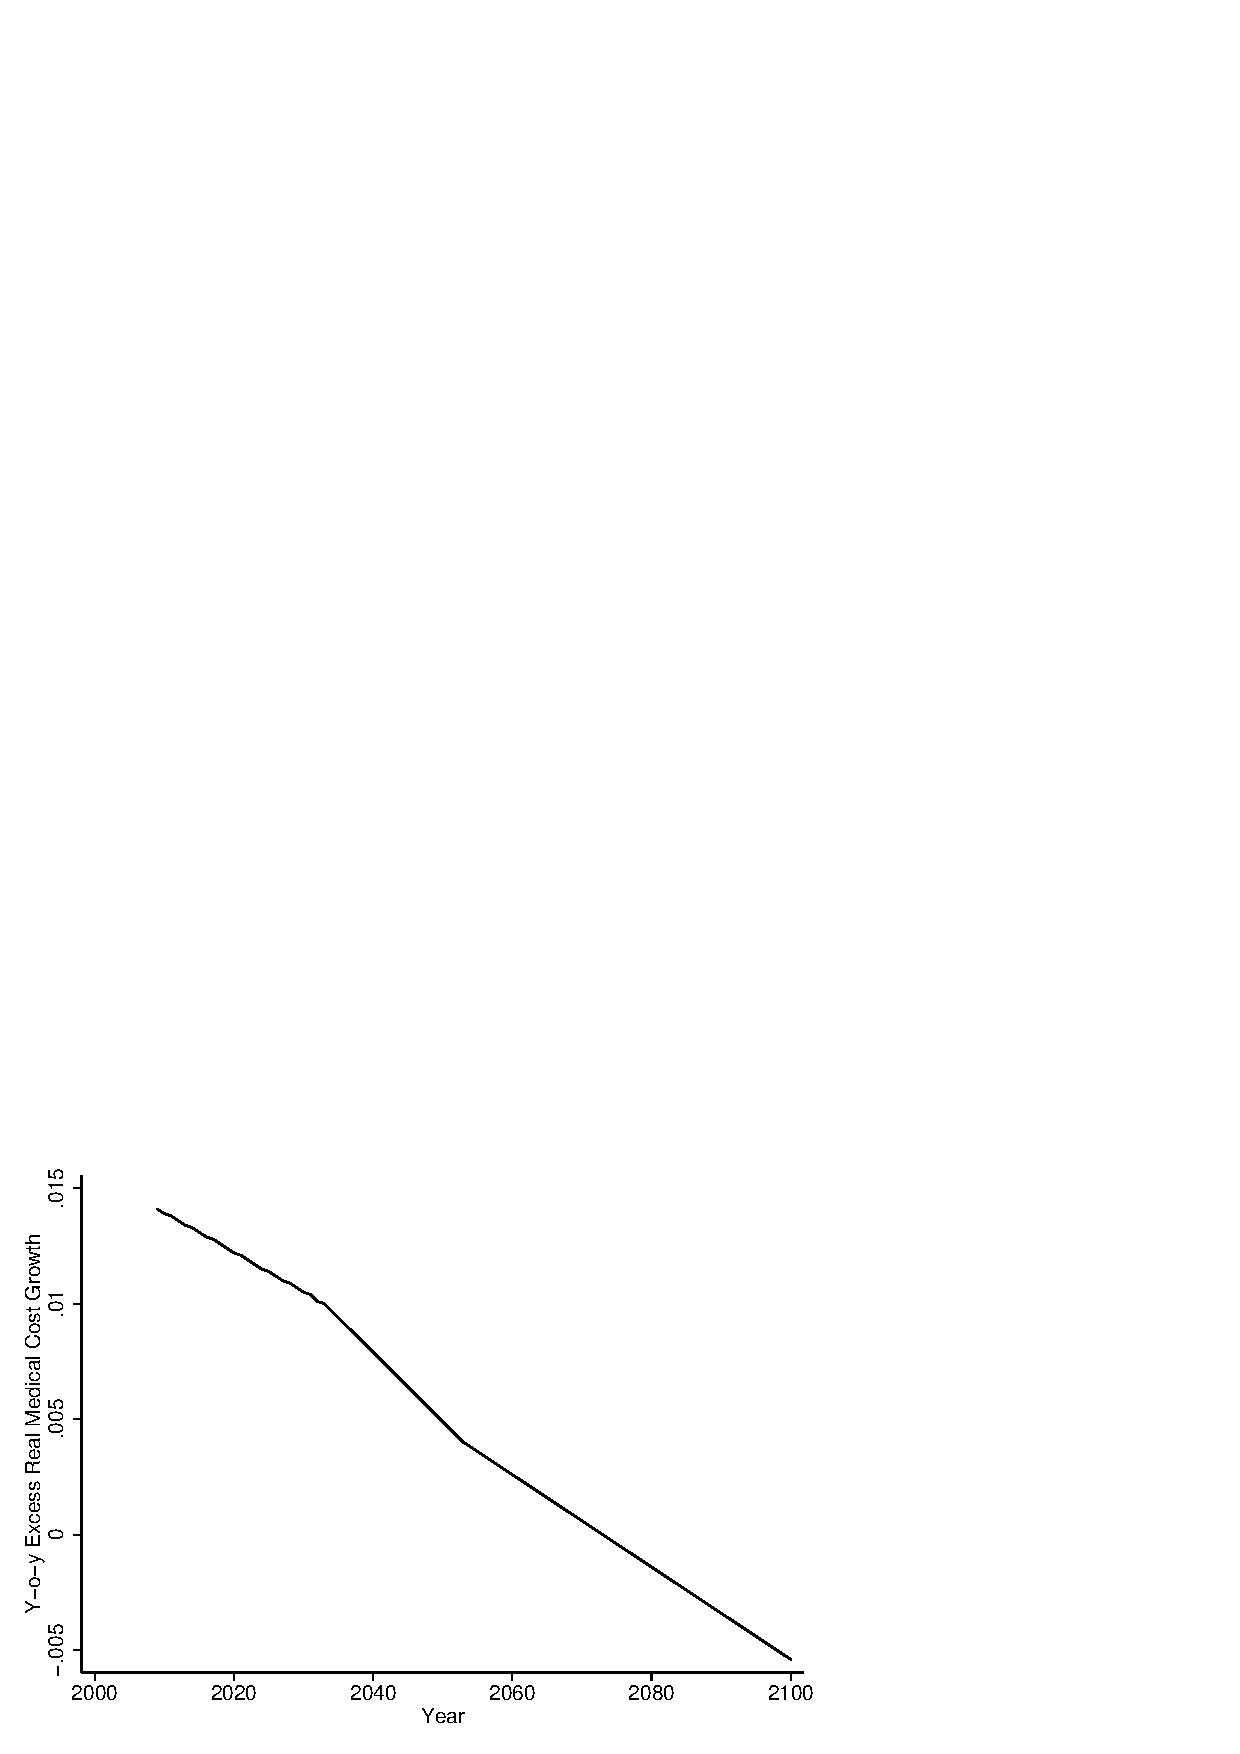
\includegraphics[height=3.5in]{AppOutput/Health/medgrowth_yearly}
\floatfoot{
\footnotesize
\noindent Sources: Congressional Budget Office, Social Security Administration.\\
\noindent Note: The year-over-year excess real medical cost growth over GDP is used to model medical cost growth in FAM.
}
\end{figure}

\noindent Medical cost growth assumptions are derived from several underlying assumptions about growth in GDP and the labor force. The real medical cost growth factor in each year is calculated by first finding the minimum of (i) the year-over-year GDP growth plus year-over-year excess medical cost growth or (ii) the Affordable Care Act cap on year-over-year medical cost growth. In order to obtain the medical cost adjustment factor for the current year of the simulation, FAM takes the cumulative product of the yearly growth factors since 2004 and then divides it by the relative growth in the labor force since 2004.\footnote{The medical cost growth assumptions come from Congressional Budget Office and SSA assumptions.
The year-over-year growth assumptions for medical costs are shown in Figure \ref{figure:medgrowth_yearly}.
The 2010-2019 GDP assumptions are based on CBO's analysis of the President's Budget, March 2009.
GDP assumptions for 2020-2100 are based on the 2008 OASDI Trustee's Report long-term projection of 2.1\% real GDP growth.}

\subsubsection{Medical Costs Before Age 30 Interview}
\label{appendix:health-costs-before-age30}

\noindent Data on utilization of medical services is sparse before the age 30 interview. There are questions about utilization in the age 12, 15, and 21 interviews along with records of births for female subjects. We combined this with information about demographics, family structure, and parents' utilization of public services to estimate medical costs at each age from 8 to 32. Models were estimated separately for males and females. All imputation and cost models are estimated using MEPS data.

\noindent Medical costs for ages 8 to 11 were estimated in three stages using age 12 interview data. First, we impute whether or not a subject spent a week in the hospital for those subjects who are missing this information in their age 12 interview. The imputation model forecasts utilization based on race and whether or not the subject was ever diagnosed with asthma between ages 8--11. Next we separate the ABC/CARE subjects into the group that spent a week in the hospital in this age range and the group that did not. For the group that did not spend any time in the hospital, we forecast medical costs as a two stage model. The first stage predicts whether there were any medical costs at all. Then, the second stage forecasts the amount of medical costs for those subjects who were predicted to have some costs. We assume the group that spent time in the hospital had some medical costs, so we skip the first stage and go directly to predicting the amount. The cost models use race, asthma diagnosis, whether or not the father was absent from the home, family use of food stamps, and number of siblings as predictors.

\noindent Medical costs for ages 12 to 14 follow a strategy similar to the age 8--11 costs. First, we impute whether or not a subject had any hospitalization for those subjects who do not report this in their age 15 interview. Imputations are based on race and presence or absence of an asthma diagnosis between ages 12--14. Again, we separated the ABC/CARE subjects into a group that had a hospitalization between age 8--11 and a group that did not. A two-stage model was used to forecast medical costs for those with no hospitalization. Medical costs for the group that had a hospitalization were estimated directly from a single-stage model. These cost models use race, asthma diagnosis, whether the mother, father, or both parents were absent from the home, family use of food stamps, and number of siblings.

\noindent To estimate medical costs for ages 15 to 20, we first impute whether or not the subject spent time in the hospital for those who are missing this information in the age 21 interview. The imputation model was based on race, asthma diagnosis between ages 15--20, and, for females, the birth of any children. The age 21 interview asks about the number of days spent in the hospital. However, it does not record the ages at which these hospital stays occurred. Considering the difficulty of assigning the hospital days to specific ages in the absence of other information, we decided to use only the indicator of whether or not there were any days spent in the hospital. Next, we separated subjects into a group that spent some time in the hospital between ages 15--20 and those who did not. As before, we used the direct model to forecast costs for those who had been to the hospital and used a two-stage model for those who had not. The cost models forecast costs based on race, asthma diagnosis, any births (female model only), use of food stamps, whether or not the subject was working age, work status, living at college, and living with parents, and marital status.

\noindent Unlike the interviews at younger ages, the age 30 interview does not ask about utilization of medical services. To estimate costs for ages 21--31, we skipped the utilization imputation step and moved directly to cost models. We used two-stage cost models. The first stage predicts whether or not there were any costs based on race, asthma diagnosis between ages 21-31, education, use of food stamps, any births (female model only), whether or not the subject was working age, living at college, living with parents, and marital status.

\noindent Table~\ref{table:pre30} summarizes individual and family characteristics used to forecast medical expenditure models for each age.

\begin{table}[H]
\begin{threeparttable}
\caption{Health Expenditure Models by Age Group, before Age 30}\label{table:pre30}
\begin{tabular}{lcccc} \toprule
Explanatory variable & \multicolumn{4}{c}{Age Group} \\
& 8-11 & 12-14 & 15-20 & 21-30 \\
\midrule
Race/ethnicity & \checkmark & \checkmark & \checkmark & \checkmark \\
Education        & $\times$ & $\times$ & $\times$ & \checkmark \\
Asthma Diagnoses & \checkmark & \checkmark & \checkmark & \checkmark \\
Hospital stays & if $\geq$ 1 week & any stay & any stay & $\times$ \\
Births & $\times$ & $\times$ & \checkmark & \checkmark \\
Mother present & $\times$ & \checkmark & $\times$ & $\times$ \\
Father present & \checkmark & \checkmark & $\times$ & $\times$ \\
Number of siblings & \checkmark & \checkmark & $\times$ & $\times$ \\
Foodstamps & \checkmark & \checkmark & \checkmark & \checkmark \\
Living arrangements & $\times$ & $\times$ & \checkmark & \checkmark \\
Working, if working age & $\times$ & $\times$ & \checkmark & \checkmark \\
\bottomrule
\end{tabular}
\begin{tablenotes}
\footnotesize
\item Note: This table summarizes the explanatory variables included in the models we use to forecast medical expenditure for each age group. Possible living arrangements are: living with parents, away at college, married, or other.\\
\end{tablenotes}
\end{threeparttable}
\end{table}

\paragraph{Specification Tests for the First-order Markov Assumption in FAM} \label{section:firstorder}

\noindent The FAM model assumes a vector first-order Markov process for health states. In Equation~\eqref{eq:trans}, $\tilde{D}_{a - \ell}$ only enters into the model when $\ell = 1$. For heart disease, hypertension, and stroke, we contrast Equation~\eqref{eq:trans} with the following extension: 

\begin{eqnarray}
I_{a,m} &=&  \bm{\mathit{1}} \left( \tilde{\bm{D}}_{0} \geq 0 \right) \bm{\Omega}_{m} + \bm{\mathit{1}} \left( \tilde{\bm{D}}_{a-1} \geq 0\right) \bm{\Lambda}_{m}  + \left( \tilde{\bm{D}}_{a-2} \geq 0\right) \tilde{\bm{\Lambda}}_{m} \nonumber \\
&+& \bm{W_a} \bm{\beta}_{m} + \bm{B} \bm{\alpha}_m + \tau(a)_m + \varepsilon_{a,m}. \label{eq:trans1}
\end{eqnarray}

We use a likelihood ratio test to test the null hypothesis $H_0: \tilde{\bm{\Lambda}}_{a,m} = \bm{0}$ in Equation~\eqref{eq:trans1}. Table~\ref{table:lrtests} show the results from these tests. For the health states considered, we do not reject the null hypothesis.

\begin{table}[H]
\begin{threeparttable}
\caption{Tests Comparing First-Order and Second Markov Processes for Disease Transition Specifications} \label{table:lrtests}
\centering
\footnotesize
\begin{tabular}{lccc}
\toprule
Statistic & LR Statistic & Degrees of Freedom & $p$-value \\
\midrule \\
Desease & \\
Heart Disease & 2.18 & 2 & 0.71 \\
Hypertension   & 0.05 & 1 & 0.83 \\
Stroke              & 3.94 & 4 & 0.14 \\
\bottomrule
\end{tabular}
\begin{tablenotes}
\footnotesize
\item Note: This table presents likelihood ratios contrasting the models in Equations~\eqref{eq:trans} and~\eqref{eq:trans1} by testing the null hypothesis $H_0: \tilde{\bm{\Lambda}}_{a,m}=0$. The variables included in the right-hand-side of each model are in Tables~\ref{table:supertab1} to~\ref{table:supertab3}. 
\end{tablenotes}
\end{threeparttable}
\end{table}

\noindent An alternative test for a first-order Markov process is the following: (i) use a linear probability model approximation to a first-order Markov process and the variables in Tables~\ref{table:supertab1} to ~\ref{table:supertab3} for each outcome of interest; (ii) calculate the correlation of the residuals with higher order lagged variables. Tables~\ref{table:1storderresidsheart} to \ref{table:1storderresidstroke} show these correlations. The results of these tests very strongly support a first-order Markov assumption.

\noindent To illustrate how to read these tests consider Table~\ref{table:1storderresidsheart}. This table reports simple first-order Pearson correlations with the indicated variable. The row presents the residuals from forecasting heart disease at age $a+1$ using different orders of lags. The estimated correlations are small.

\begin{landscape}
\begin{table}[H]
\begin{threeparttable}
\caption{Tests for Linear Probability Forecasts of Heart Disease at $a+1$} \label{table:1storderresidsheart}
\scriptsize
\centering
\begin{tabular}{lcccccccccc} \toprule
& \multicolumn{10}{c}{Residuals of Forecast of Heart Disease at age $a+1$} \\
Correlations with	&	Predictor Diabetes &	Hypertension &	Diabetes &	Hypertension &	Diabetes	&	Hypertension &	Diabetes & Hypertension & Diabetes & Hypertension \\
                    &	at $a - 2$ &	at $a - 2$		&	at $a - 3$ & at $a - 3$		& at $a - 4$		& at $a - 4$		& at $a - 5$	& at $a - 5$	& at $a - 6$	& at $a - 6$	\\

\midrule \\
&	-0.002	&	-0.006	&	-0.004	& -0.009 &	-0.017	& -0.020	&	-0.015	&	-0.017 &-0.009	&	0.004	\\
\bottomrule
\end{tabular}
\begin{tablenotes}
\footnotesize
\item Note: This table presents the correlation between the residuals from forecasting heart disease at age $a+1$ and the predictors indicated in each column.
\end{tablenotes}
\end{threeparttable}
\end{table}

\begin{table}[H]
\begin{threeparttable}
\caption{Tests for Linear Probability Forecasts of Hypertension at $a+1$} \label{table:1storderresidshyper}
\centering
\scriptsize
\begin{tabular}{lccccc} \toprule
& \multicolumn{5}{c}{Residuals of Forecast of Hypertension at age $a+1$} \\
Correlations with	&	Predictor Diabetes & Diabetes & Diabetes & Diabetes & Diabetes 	\\
                    & at $a - 2$	& at $a - 3$	& at $a - 4$	& at $a - 5$	& at $a - 6$	\\
\midrule
&	0.003	& 0.009	&	0.012	&	0.008	&	0.001	\\
\bottomrule
\end{tabular}
\begin{tablenotes}
\footnotesize
\item Note: This table presents the correlation between the residuals from forecasting hypertension at age $a+1$ and the predictors indicated in each column.
\end{tablenotes}
\end{threeparttable}
\end{table}

\begin{table}[H]
\begin{threeparttable}
\caption{Tests for Linear Probability Forecasts of Stroke at $a+1$} \label{table:1storderresidstroke}
\centering
\footnotesize
\begin{tabular}{l *{8}{c}}
\toprule
& \multicolumn{8}{c}{Residuals of Forecast of Stroke at age $a+1$} \\
Correlations with	&	Predictor Cancer &	Diabetes & Heart Disease &	Hypertension &	Cancer	& Diabetes & Heart Disease & Hypertension  \\
                    &	at $a-2$	&	at $a - 2$ & at $a - 2$	& at $a - 2$	& at $a-3$	& at $a - 3$	& at $a - 3$	& at $a - 3$ \\
\midrule \\
&	0.004 &	0.008	&	0.001	&	0.001	&	-0.002	&	0.017 &	-0.004 &	-0.001	\\
\bottomrule
\end{tabular}
\begin{tablenotes}
\footnotesize
\item Note: This table presents the correlation between the residuals from forecasting stroke at age $a+1$ and the predictors indicated in each column.
\end{tablenotes}
\end{threeparttable}
\end{table}
\end{landscape}
